\section{Testing}
\label{secD4:Testing}

In questo capitolo sono descritti i casi di testing effettuati sulle APIs da noi sviluppate. La parte di testing è fondamentale per poter individuare eventuali problemi sulle APIs sviluppate e accertarsi che tutto funzioni secondo quello voluto.\\
Prima di andare con la descrizione dei vari casi di testing effettuati, si specifica che per comodità siamo andati a suddividere i testing in base a quale resource riguardassero, quindi utente, calendario ed evento e in base alla tipologia di API da testare, ovvero POST, PUT e GET. Inoltre, prima di ciascuna procedura di testing per ogni API, sono presenti delle procedure necessarie affinché si possa effettuare con successo un certo testing per una API. Ad esempio, prima di tutto, nella funzione "beforeAll()" di ciascun file, si sono creati degli oggetti che ci servivano per poter testare con successo le APIs, come "userId" duplicati, "userId" (parametro essenziale, che deve essere sempre presente per far funzionare un' API) corretti, calendari da cui ottenere l' "IDCalendario" (essenziale, come vedremo, per il POST e il PUT dell'evento e per il PUT del calendario), eventi da cui ottenere l' "IDEvento" (essenziale, come vedremo, per il PUT evento), calendari pieni e vuoti di eventi (essenziale per l'api GET Eventi), ecc.. E dopo, alla fine della procedura di testing per una certa API, abbiamo sempre inserito nell' "afterAll()" la pulizia di tutto il database MongoDB, in modo tale che gli altri testing non avessero conflitti con quello fatto in altri file di testing. \\ Nelle seguenti pagine, si può ottenere un resoconto dei testing effettuati: \href{https://plan-it.it/test-report.html} {https://plan-it.it/test-report.html}, \href{https://api.plan-it.it/coverage/index.html} {https://api.plan-it.it/coverage/index.html}. Nel secondo link, è presente il documento html, che è stato mostrato anche in aula, che ci è stato consigliato di aggiungere. Aprendo quest'ultimo link, si può notare che non tutte le linee sono state coperte per ciascun file esaminato, perché? I motivi sono molto semplici; infatti tutte le linee non coperte riguardano o la funzione "handle()", presente in ciascun file delle APIs, che è una funzione che viene invocata quando si vuole invocare un'API, ma per i casi di test abbiamo deciso di invocare direttamente le APIs, invece che gli handler, in quanto questi, nei test, davano dei problemi, o pezzi di codice in cui sono presenti controlli ad errori da noi non verificabili. Per l'appunto, in tutti i file, le parti di codice in cui sono presenti il "throw" del codice "500" e "501" non sono da noi verificabili, in quanto sono errori derivanti da errori generici che spuntano durante l'esecuzione dell'API, oppure dalla sconnessione improvvisa dal server MongoDB; tutte condizioni da noi non replicabili nei test. Quindi, queste sono le ragioni per cui, nel secondo link riportato, e nella foto sottostante, la percentuale coperta di "lines" per ciascuna cartella è, quasi in tutti i casi, diversa dal 100\%.

\begin{center}
        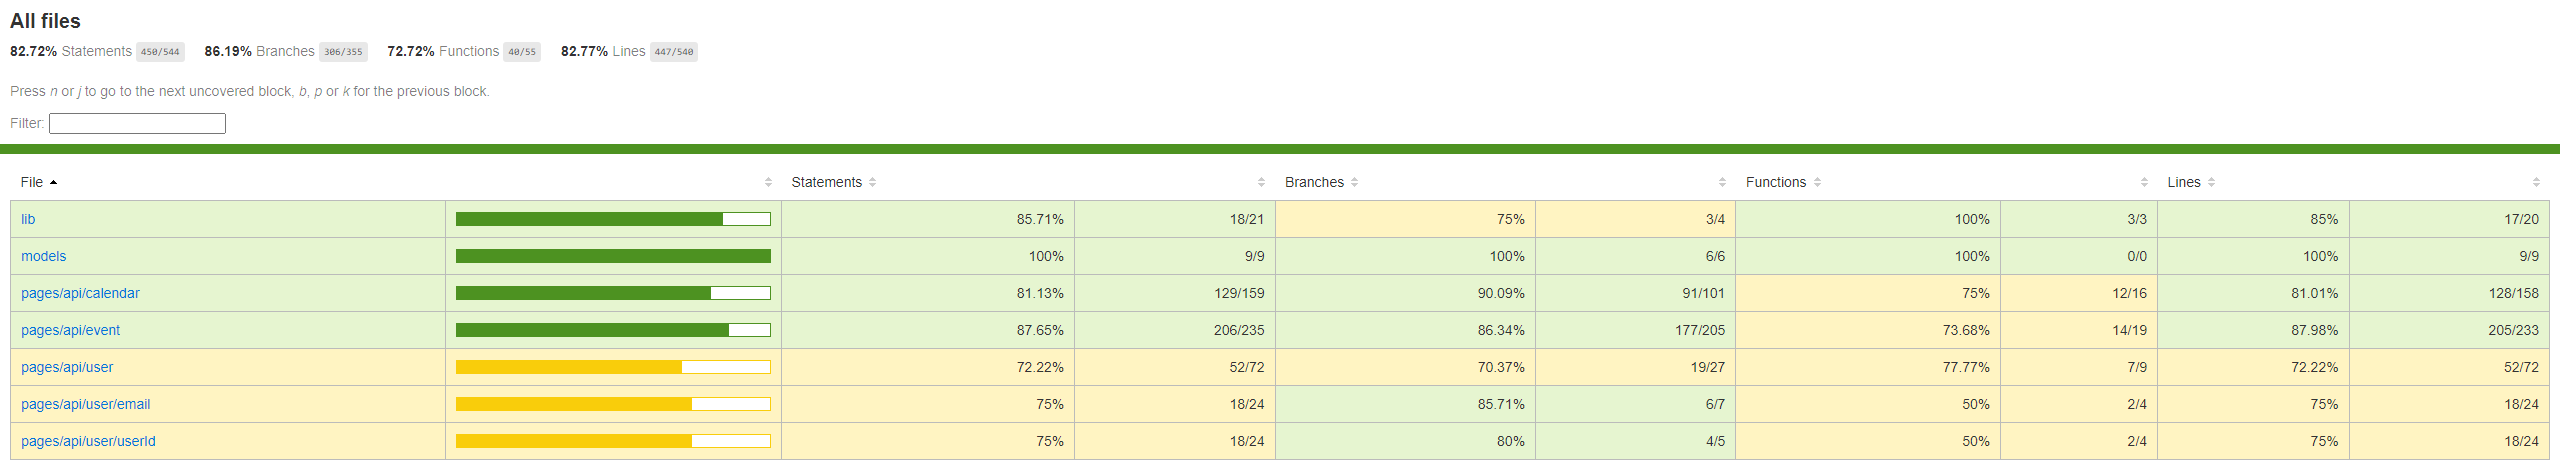
\includegraphics[width=1\textwidth, height=0.1\textheight]{img/png/tests/test_totale_1.png}
        \blfootnote{Immagine \href{https://github.com/Life-planner/Documentazione/blob/main/D4/img/png/tests/test_totale_1.png}{PNG} Resoconto testing, secondo link dato}
        \captionof{figure}{Resoconto testing, secondo \href{https://api.plan-it.it/coverage/index.html} {link} dato}
\end{center}

Abbiamo deciso anche di produrre un secondo resoconto, reperibile a questo \href{https://plan-it.it/test-report.html} {link}, in quanto quest'ultimo ci sembrava migliore per mostrare tutti i test cases effettuati, con la loro relativa breve descrizione per far intendere a cosa ci riferissimo. Per questo motivo, useremo questo resoconto nelle prossime immagini.


\begin{listaPersonale}{TS}
        \elemento [Evento - POST] {ts:eventoPost}
                Come già detto precedentemente in \ref{apd:creaEvento}, i parametri che sono obbligatori per non ottenere l'errore "400 - IDCalendario or titolo or evento details missing" da questa API sono "userId", "IDCalendario", "titolo", "isEventoSingolo" e "eventoSingolo" o "eventoRipetuto" ("eventoSingolo" quando "isEventoSingolo" = true, "eventoRipetuto" se "isEventoSingolo" = false). Per questo motivo i primi due test effettuati, sono stati fatti mandando in input solo questi parametri scritti con il loro giusto formato, in modo tale di non ottenere l'errore "409 - Wrong format for (parameter with wrong format)" e ottenere il buon esito dall'esecuzione dell'API con l'arrivo del codice "200" e il messaggio "Event inserted correctly", come è avvenuto infatti. Sono stati citati "due test" iniziali, in quanto il primo è stato fatto con "eventoSingolo" != null e "isEventoSingolo" = true, e il secondo invece con "eventoRipetuto" != null e "isEventoSingolo" = false. Questi due test sono i test con il minor numero possibile di parametri che si possono avere per avere un possibile buon esito dall'esecuzione dell' API, sempre se anche gli altri controlli citati in \ref{apd:creaEvento} vengono superati.
                A partire da questi due test, sono stati fatti tutti gli altri test, in cui mano a mano si sono inseriti anche gli altri parametri opzionali, con formati corretti, che possono essere presenti come input per l'API "creaEvento" (\ref{apd:creaEvento}) nelle loro varie combinazioni, osservando se si ottenesse sempre il successo ("200 - event inserted correctly"). I parametri opzionali inseriti nelle varie combinazioni sono "luogo", "priorita", "difficolta", "notifiche" e "durata". Si è deciso di fare tutti i possibili casi con le varie combinazioni, anche sapendo da altri test già fatti, che il risultato sarebbe stato corretto, per poter osservare che tutto andasse come aspettato con tutte le varie possibilità e anche poter identificare più velocemente le cause di errore, nel caso in cui i test non fossero andati a buon fine. Infatti in tutti i primi test, ciò che volevamo ottenere era il buon esito dell'esecuzione dell' API "creaEvento" con "200 - Event inserted correctly".
                \begin{center}
                        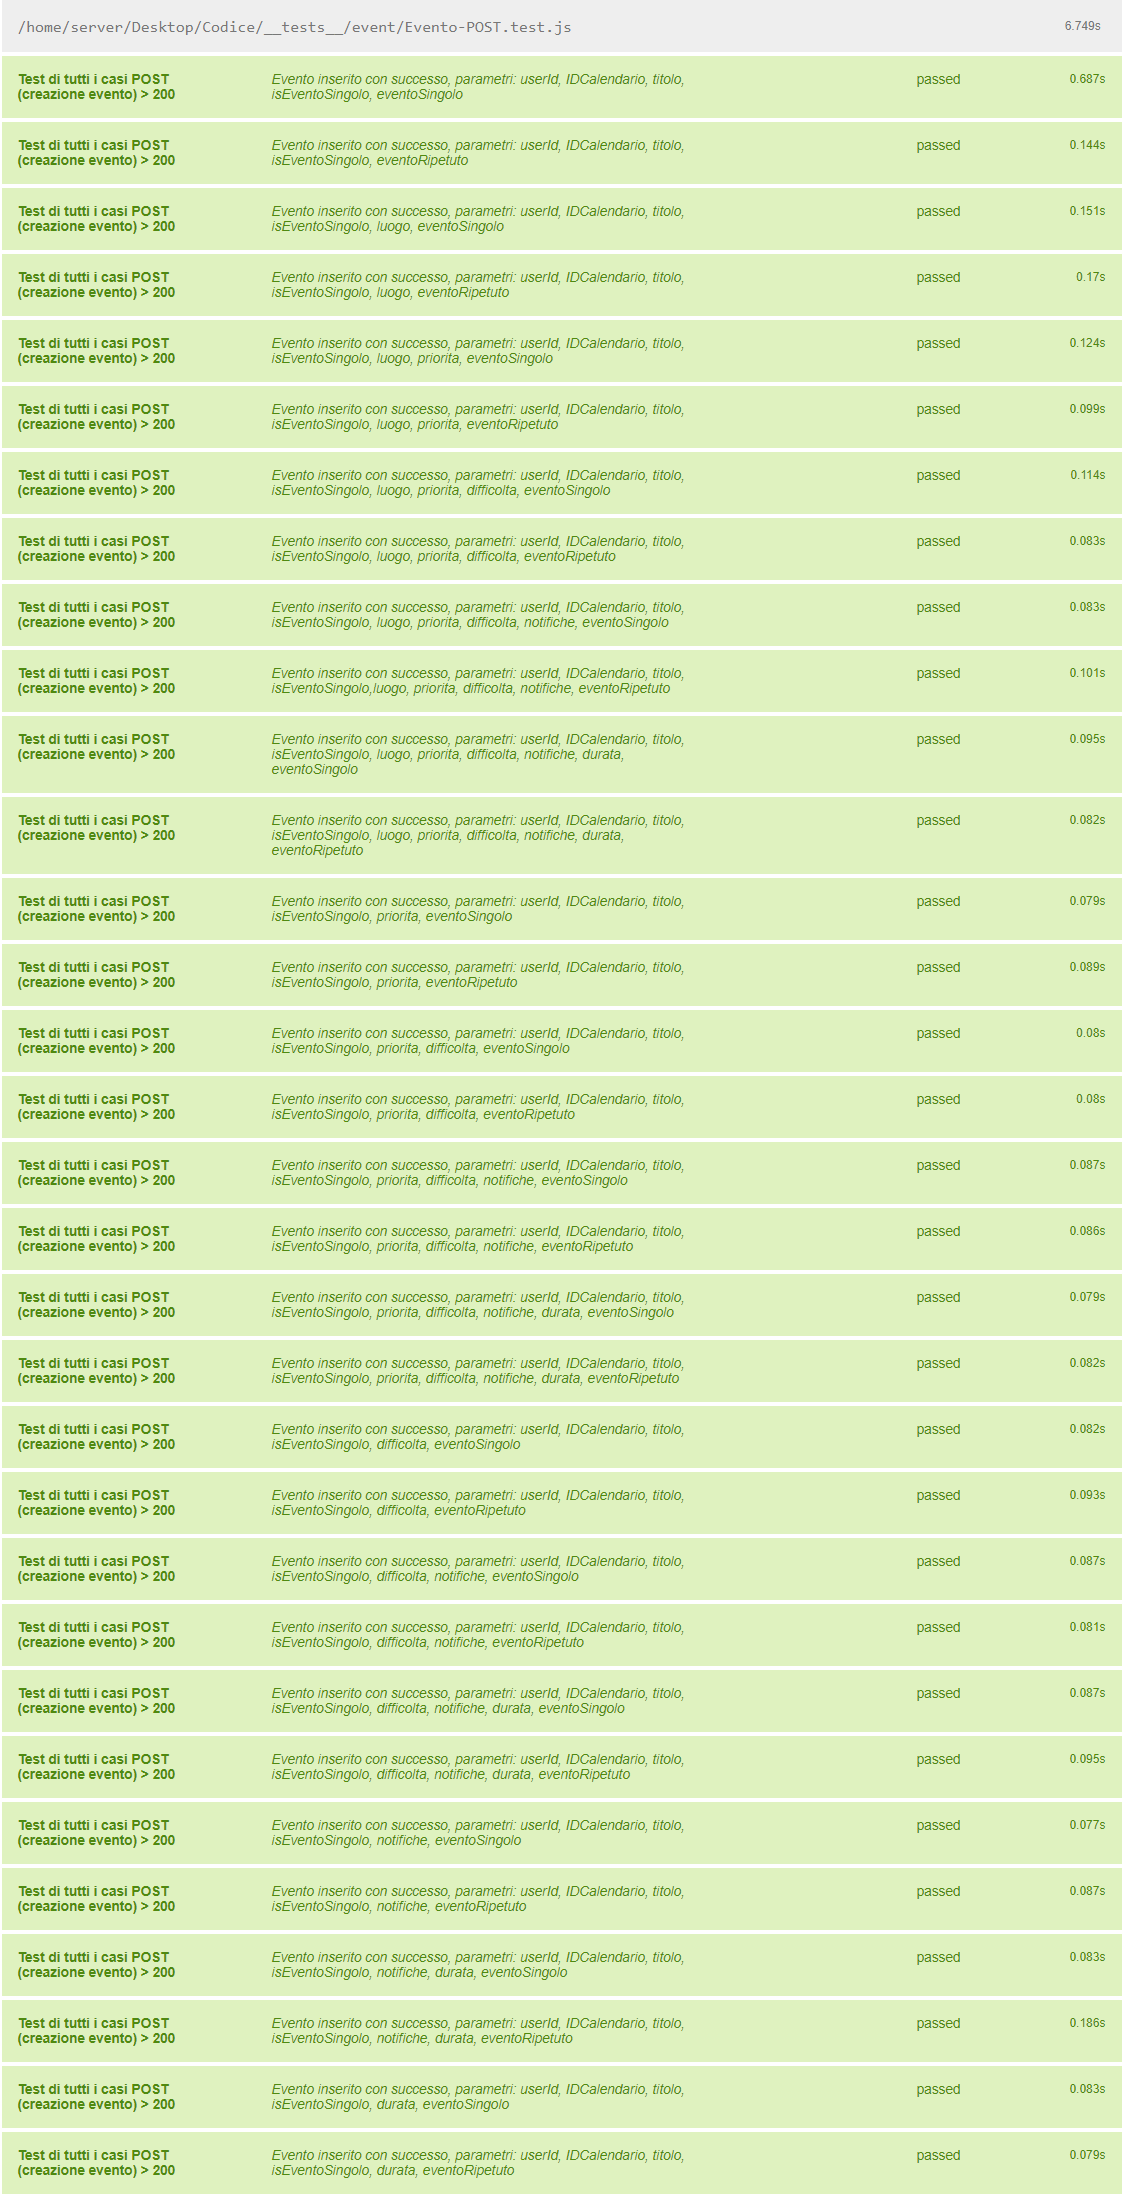
\includegraphics[width=0.5\textwidth, height=0.6\textheight]{img/png/tests/EventoPost/200_PostEvento.png}
                        \blfootnote{Immagine \href{https://github.com/Life-planner/Documentazione/blob/main/D4/img/png/tests/EventoPost/200_PostEvento.png}{PNG} Casi 200, POST Evento}
                        \captionof{figure}{Casi 200, POST evento}
                \end{center}
                Dal test numero 32 al 38 ("Test di tutti i casi POST (creazione evento) > 400", "Manca uno o piu parametri -- IDCalendario, parametri presenti: userId, titolo, isEventoSingolo, eventoSingolo"), abbiamo formulato test con lo scopo di ottenere errori del tipo "400 - Parameter missing" per poter osservare se i controlli presenti all'interno dell'API fossero corretti e identificassero che tutti i parametri necessari, affinché l'API possa eseguire con successo, fossero presenti. Come si può notare in questa \href{https://plan-it.it/test-report.html} {pagina} e nell'immagine sottostante, tutti questi casi sono stati passati con successo dal codice dell'API "creaEvento" per tutti i possibili parametri obbligatori che possono mancare, ovvero: "userId", "titolo", "isEventoSingolo", "eventoSingolo" o "eventoRipetuto".
                \begin{center}
                        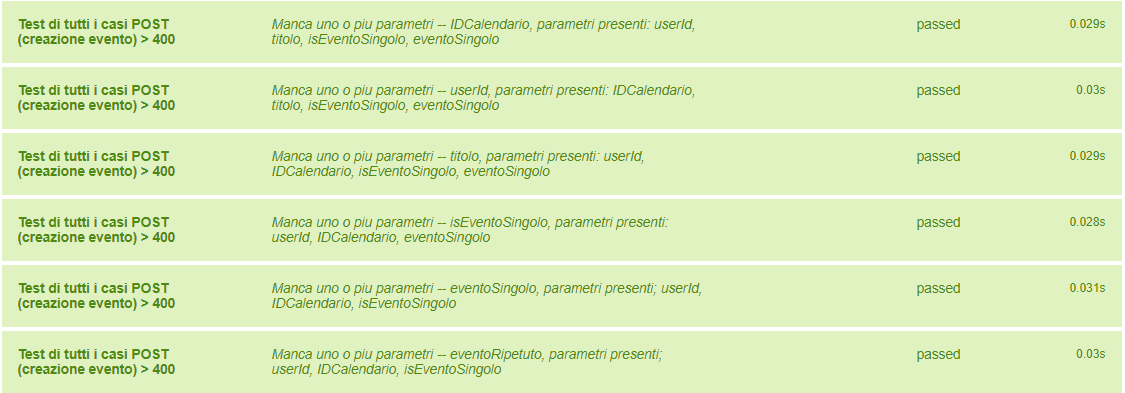
\includegraphics[width=1\textwidth, height=0.25\textheight]{img/png/tests/EventoPost/400_missingParameter_PostEvento.png}
                        \blfootnote{Immagine \href{https://github.com/Life-planner/Documentazione/blob/main/D4/img/png/tests/EventoPost/400_missingParameter_PostEvento.png}{PNG} Casi 400 "Parameter missing", POST Evento}
                        \captionof{figure}{Casi 400 "Parameter missing", POST Evento}
                \end{center}
                Dal test case numero 39, si è voluto controllare che i controlli riguardo al formato dei parametri inseriti funzionassero. Infatti nel caso in cui, uno dei parametri inseriti avesse un formato scorretto, si deve ottenere l'errore "400 - Wrong format for (parameter)". Questi controlli riguardo al formato scorretto sono fatti per i seguenti parametri: "luogo", "priorita", "difficolta", "notifiche", "durata", "eventoSingolo" ed "eventoRipetuto". Come si può notare dalla lista di test effettuati, sono stati fatti più test anche sullo stesso parametro sempre ottenendo questo errore, per poter osservare se l'API identificasse sempre l'errore con i vari casi con cui un parametro può assumere un valore erroneo.
                \begin{center}
                        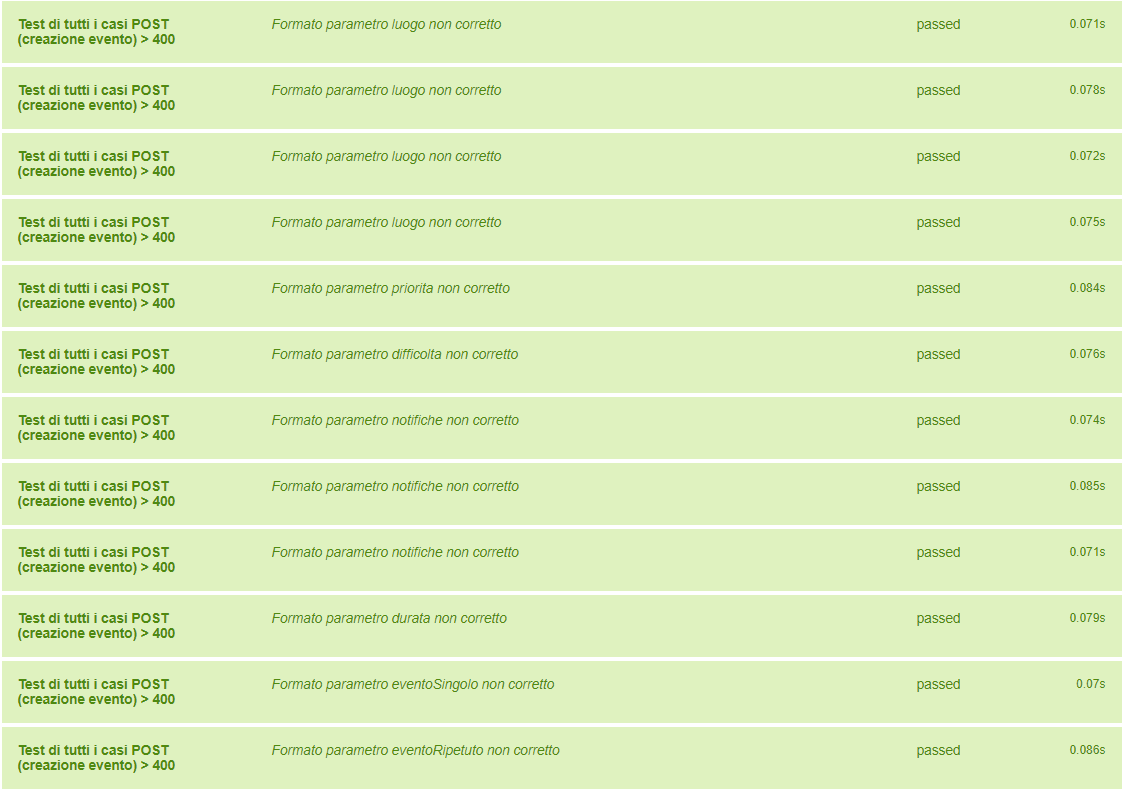
\includegraphics[width=0.9\textwidth, height=0.4\textheight]{img/png/tests/EventoPost/400_wrongFormat_PostEvento.png}
                        \blfootnote{Immagine \href{https://github.com/Life-planner/Documentazione/blob/main/D4/img/png/tests/EventoPost/400_wrongFormat_PostEvento.png}{PNG} Casi 400 "Wrong format for (parameter)", POST Evento}
                        \captionof{figure}{Casi 400 "Wrong format for (parameter)", POST Evento}
                \end{center}
                Invece, dal test case numero 51, si è controllato che i casi in cui si inserisse un "userId" scorretto, ovvero che o non esistesse nel database MongoDB o fosse un duplicato, fossero individuati e fosse mandato il rispettivo messaggio di errore. Infatti, come si può notare dal codice presente nella cartella "\_tests\_" della repo "Codice" (\href{https://github.com/Life-planner/Codice/tree/main/__tests__}{cartella "tests"}), prima dell'esecuzione di tutti i vari test per "creaEvento" è stato creato un "userId" corretto ("utenteTestEventoPOST"), che è stato usato in tutti i vari casi in cui non volevamo ottenere un errore ottenuto da questo parametro e un "userId" duplicato ("utenteTestEventoPOSTDuplicato"). Quest'ultimo è stato utilizzato come parametro erroneo, per vedere se l'API lo individuasse e inviasse l'errore "409 - There are too many users with that userId", come è successo. Invece, è stato usato l' "userId" "UtenteNonEsiste", ma andava bene un qualsiasi altro "userId" che non fosse salvato nel database, per vedere se il controllo, riguardo se l' "userId" esistesse o meno, funzionasse e ottenessimo l'errore "409 - There is no user with that userId", come è successo.
                \begin{center}
                        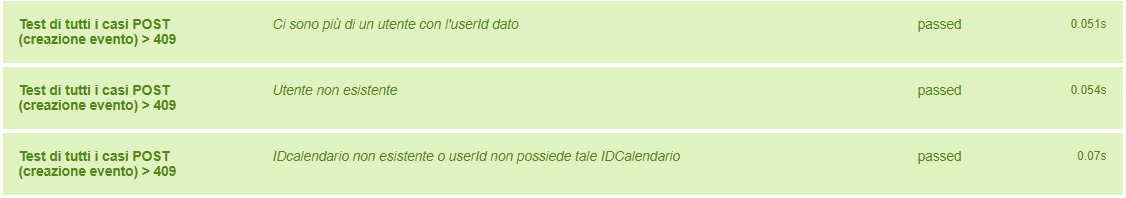
\includegraphics[width=1\textwidth, height=0.12\textheight]{img/png/tests/EventoPost/409_PostEvento.png}
                        \blfootnote{Immagine \href{https://github.com/Life-planner/Documentazione/blob/main/D4/img/png/tests/EventoPost/409_PostEvento.png}{PNG} Casi 409, POST Evento}
                        \captionof{figure}{Casi 409, POST Evento}
                \end{center}
        \elemento [Evento - PUT] {ts:eventoPut}
                Questa API, come già anticipato in \ref{apd:modificaEvento}, ha bisogno di tutti gli attributi che formano la struttura dati "Evento" come parametri per iniziare la sua procedura. Nel caso in cui mancasse uno dei seguente attributi, ovvero "IDEvento" ("id" dell'evento che si sta modificando), "userId", "titolo", "isEventoSingolo", "luogo", "priorita", "difficolta", "notifiche", "data", "durata", "eventoSingolo" e "eventoRipetuto", si ottiene l'errore "400 - Parameter missing". Quindi, nei primi due test effettuati, che hanno l'obiettivo di ottenere il codice di successo "200" con messaggio "Event edited correctly", si è mandato in input tutti questi parametri, con l'unica differenza che nel primo abbiamo messo "isEventoSingolo" = true, dunque l'evento è un evento singolo, invece nel secondo "isEventoSingolo" = false, dunque l'evento è un evento ripetuto. Per ottenere "200", questi sono gli unici due casi distinti, quindi abbiamo fatto questi, e abbiamo ottenuto, come sperato, "200" con messaggio "Event edited correctly", come si può notare nella foto sottostante o in questa  \href{https://plan-it.it/test-report.html} {pagina}.
                \begin{center}
                        \includegraphics[width=1\textwidth, height=0.1\textheight]{img/png/tests/EventoPut/200_PutEvento.png}
                        \blfootnote{Immagine \href{https://github.com/Life-planner/Documentazione/blob/main/D4/img/png/tests/EventoPut/200_PutEvento.png}{PNG} Casi 200, PUT Evento}
                        \captionof{figure}{Casi 200, PUT evento}
                \end{center}
                In seguito, abbiamo fatto tredici test che avevano lo scopo di ottenere il codice "400" con il messaggio "Parameter missing"; infatti in questi tredici test, siamo andati a togliere in ciascun test, un diverso parametro in modo tale da osservare se l'API individuasse correttamente la mancanza di ciascun parametro. In questa \href{https://plan-it.it/test-report.html} {pagina} e nella foto sottostante, si può notare che i test sono stati effettuati con successo e che l'API ha notato la mancanza del parametro da noi appositamente tolto, inviando in output il codice "400" con il messaggio di errore "Parameter missing".
                \begin{center}
                        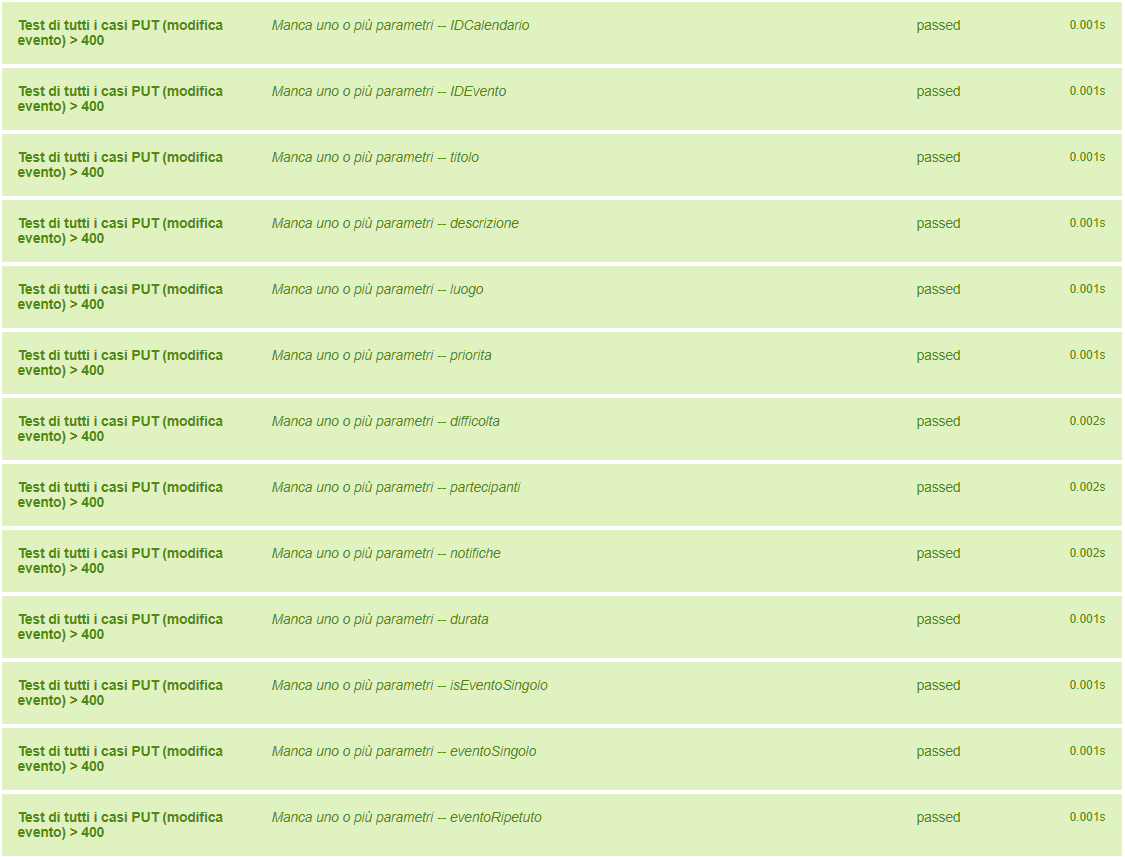
\includegraphics[width=0.8\textwidth, height=0.37\textheight]{img/png/tests/EventoPut/400_missingParameter_PutEvento.png}
                        \blfootnote{Immagine \href{https://github.com/Life-planner/Documentazione/blob/main/D4/img/png/tests/EventoPut/400_missingParameter_PutEvento.png}{PNG} Casi 400, PUT Evento}
                        \captionof{figure}{Casi 400 "Parameter missing", PUT Evento}
                \end{center}
                Dal test numero 15, siamo andati a fare degli input appositi, che avevano lo scopo di ottenere il codice "400" con il messaggio di errore "Wrong format for (parameter)";  infatti gli attributi "luogo", "priorita", "difficolta", "notifiche", "durata", "eventoSingolo" ed "eventoRipetuto", possono essere inviati con dei formati sbagliati, ovvero possono avere dei valori o una sintassi sbagliata. Dunque, in questi sette test, che si possono guardare dalla foto sottostante o da questa \href{https://plan-it.it/test-report.html} {pagina}, siamo andati a inviare in input un parametro, scelto una alla volta tra gli attributi sopra citati, con formato erroneo. Come era aspettato, l'API si è comportata correttamente, inviandoci in output il codice "400" con il messaggio di errore "Wrog format for (parameter)".
                \begin{center}
                        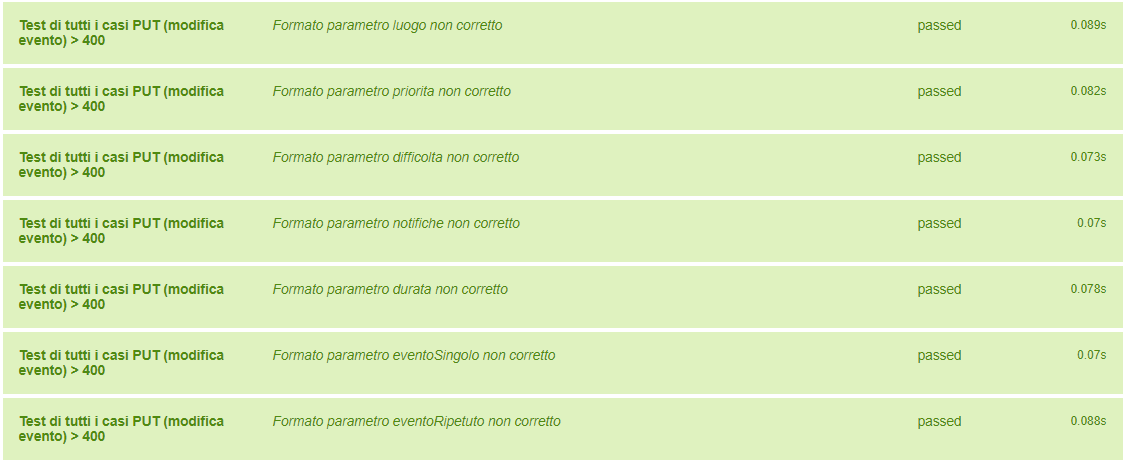
\includegraphics[width=1\textwidth, height=0.27\textheight]{img/png/tests/EventoPut/400_wrongFormat_PutEvento.png}
                        \blfootnote{Immagine \href{https://github.com/Life-planner/Documentazione/blob/main/D4/img/png/tests/EventoPost/400_wrongFormat_PostEvento.png}{PNG} Casi 400 "Wrong format for (parameter)", PUT Evento}
                        \captionof{figure}{Casi 400 "Wrong format for (parameter)", PUT Evento}
                \end{center}
                In due test, siamo andati a testare che con l'invio di un "userId" sbagliato, ovvero o non esistente o duplicato, l'API lo notasse e inviasse un codice di errore "409" con messaggio "There is no user with that userId" oppure "There are too many users with that userId" rispettivamente. Come si può notare, l'API si è comportata correttamente inviandoci gli output sopra citati. Sottolineiamo che questi controlli fatti sull' "userId" sono gli stessi presenti in \ref{ts:eventoPost}, quindi questi test non sono altro che una conferma che questi controlli funzionano sempre correttamente.
                \begin{center}
                        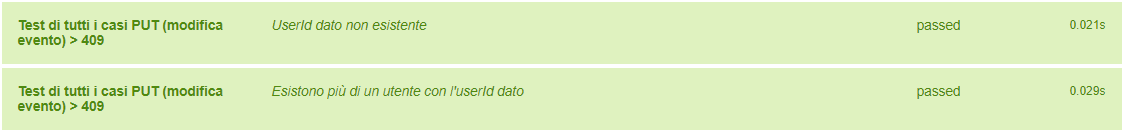
\includegraphics[width=1\textwidth, height=0.08\textheight]{img/png/tests/EventoPut/409_userId_PutEvento.png}
                        \blfootnote{Immagine \href{https://github.com/Life-planner/Documentazione/blob/main/D4/img/png/tests/EventoPut/409_userId_PutEvento.png}{PNG} Casi 409 riguardo "userId", PUT Evento}
                        \captionof{figure}{Casi 409 riguardo "userId", PUT Evento}
                \end{center}
                Nei restanti test, siamo andati a testare i casi in cui l' "IDCalendario" o l' "IDEvento" fossero sbagliati, ovvero o non esistenti o non appartenenti all' "userId" inviato in input. Nel primo test ,che si può leggere nella foto sottostante, abbiamo inviato un "IDCalendario" che non facesse parte della lista di calendari di quell' "userId" indicato, e come aspettato, abbiamo ricevuto il codice "409" con il messaggio di errore "There is no calendar with that ID or you do not own the calendar". Nell'ultimo test abbiamo inviato un "IDEvento" che non apparteneva alla lista di eventi dell' "userId" e abbiamo ricevuto, come aspettato, il codice "409" con il messaggio "You do not own the event".  Dunque, tutti i test effettuati hanno avuto successo anche per questa API.
                \begin{center}
                        \includegraphics[width=1\textwidth, height=0.08\textheight]{img/png/tests/EventoPut/409_PutEvento.png}
                        \blfootnote{Immagine \href{https://github.com/Life-planner/Documentazione/blob/main/D4/img/png/tests/EventoPut/409_PutEvento.png}{PNG} Casi 409, PUT Evento}
                        \captionof{figure}{Casi 409, PUT Evento}
                \end{center}
        \elemento [Evento - DELETE] {ts:eventoDelete}
                Questa API ha bisogno (come già scritto in \ref{apd:eliminaEvento}), dell' "IDEvento" dell'evento  che si vuole eliminare con l' "userId" dell'utente che ha tale evento. Dunque, nel primo test, in cui volevamo ottenere il codice "200" con messaggio di successo "Event deleted correctly", abbiamo inserito questi parametri scritti correttamente, che, quindi, potessero superare anche gli altri controlli presenti nell' API. Come previsto, da questo test abbiamo ottenuto il codice e messaggio sopra citati.
                \begin{center}
                        \includegraphics[width=1\textwidth, height=0.08\textheight]{img/png/tests/EventoDelete/200_DeleteEvento.png}
                        \blfootnote{Immagine \href{https://github.com/Life-planner/Documentazione/blob/main/D4/img/png/tests/EventoDelete/200_DeleteEvento.png}{PNG} Casi 200, DELETE Evento}
                        \captionof{figure}{Casi 200, DELETE evento}
                \end{center}
                Nei seguenti casi, siamo andati a controllare che nel caso in cui non inserissimo uno dei parametri sopra citati, l'API lo notasse e ci inviasse il codice "400" con messaggio di errore "Parameter missing", cosa che è avvenuta sia nel caso in cui mancava "userId" sia nel caso in cui mancava "IDEvento".
                \begin{center}
                        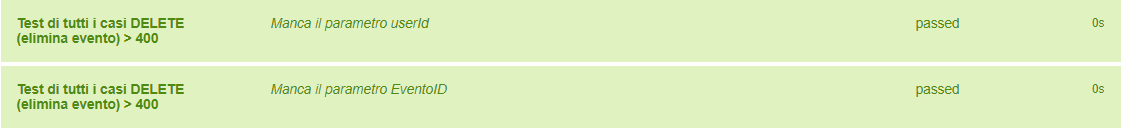
\includegraphics[width=1\textwidth, height=0.08\textheight]{img/png/tests/EventoDelete/400_missingParameter_deleteEvento.png}
                        \blfootnote{Immagine \href{https://github.com/Life-planner/Documentazione/blob/main/D4/img/png/tests/EventoDelete/400_missingParameter_deleteEvento.png}{PNG} Casi 400 "Parameter missing", DELETE Evento}
                        \captionof{figure}{Casi 400 "Parameter missing", DELETE Evento}
                \end{center}
                In seguito, abbiamo fatto, come in \ref{ts:eventoPost}, i due test in cui inseriamo un "userId" scorretto, ovvero o duplicato o non esiste, aspettandoci il codice "409" con i messaggi "There are too many users with that userId" e "There is no user with that userId" rispettivamente. E, come avvenuto in \ref{ts:eventoPost}, i due test sono avvenuti con successo, ottenendo i codici e messaggi sopra citati.
                \begin{center}
                        \includegraphics[width=1\textwidth, height=0.08\textheight]{img/png/tests/EventoDelete/409_userId_DeleteEvento.png}
                        \blfootnote{Immagine \href{https://github.com/Life-planner/Documentazione/blob/main/D4/img/png/tests/EventoDelete/409_userId_DeleteEvento.png}{PNG} Casi 409 riguardo "userId", DELETE Evento}
                        \captionof{figure}{Casi 409 riguardo "userId", DELETE Evento}
                \end{center}
                L'ultimo caso testato è quello in cui si inserisce un "IDEvento" che non esiste tra gli "id" degli eventi appartenenti all' "userId" dato. In questo caso, prevediamo di ottenere il codice "409" con il messaggio di errore "You do not own the event", cosa che è avvenuta; quindi, anche questo test è andato a buon fine.
                \begin{center}
                        \includegraphics[width=1\textwidth, height=0.04\textheight]{img/png/tests/EventoDelete/409_DeleteEvento.png}
                        \blfootnote{Immagine \href{https://github.com/Life-planner/Documentazione/blob/main/D4/img/png/tests/EventoDelete/409_DeleteEvento.png}{PNG} Casi 409, DELETE Evento}
                        \captionof{figure}{Casi 409, DELETE Evento}
                \end{center}
        \elemento [Eventi - GET] {ts:eventiGet}
                Come già detto in \ref{apd:getEventi}, lo scopo di questa API è di ritornare l'array di eventi che fanno parte di un calendario. Dunque, i parametri necessari, affinché questa procedura possa andare, sono "IDCalendario" del calendario di cui si vogliono ottenere i suoi eventi e l' "userId" dell'utente che ha tale calendario. Per questo motivo, nel primo caso di test, in cui avevamo l'obiettivo di ottenere "200" con il ritorno dell'array di eventi, abbiamo inserito i parametri sopra citati corretti, in modo tale che superassero anche gli altri controlli. Come aspettato, abbiamo ottenuto il codice sopra citato e il test è andato a buon fine.
                \begin{center}
                        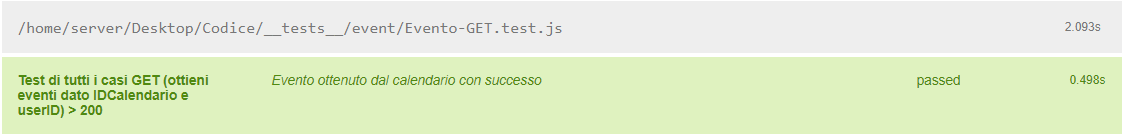
\includegraphics[width=1\textwidth, height=0.07\textheight]{img/png/tests/EventoGet/200_getEventi.png}
                        \blfootnote{Immagine \href{https://github.com/Life-planner/Documentazione/blob/main/D4/img/png/tests/EventoGet/200_getEventi.png}{PNG} Casi 200, GET eventi}
                        \captionof{figure}{Casi 200, GET Eventi}
                \end{center}
                Nei successivi due test, siamo andati a togliere una alla volta i parametri "userId" e "IDCalendario" dai parametri in input, in modo tale da controllare che l'API notasse tale mancanza e ce la segnalasse con un codice di ritorno "400" e il messaggio "Parameter missing", cosa che è successa in entrambii casi; cosa che si può notare dalla foto sottostante o da questa \href{https://plan-it.it/test-report.html} {pagina}.
                \begin{center}
                        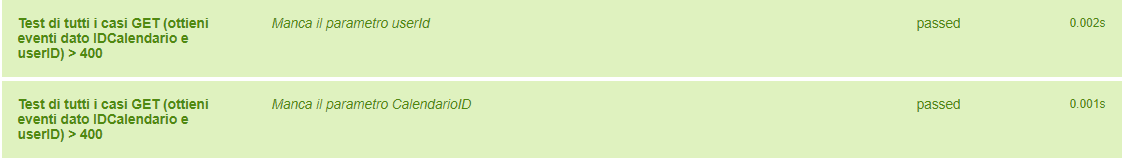
\includegraphics[width=1\textwidth, height=0.09\textheight]{img/png/tests/EventoGet/400_missingParameter_getEventi.png}
                        \blfootnote{Immagine \href{https://github.com/Life-planner/Documentazione/blob/main/D4/img/png/tests/EventoGet/400_missingParameter_getEventi.png}{PNG} Casi 400 "Parameter missing", GET Eventi}
                        \captionof{figure}{Casi 400 "Parameter missing", GET Eventi}
                \end{center}
                Come sempre, abbiamo messo i due casi in cui l' "userId" era scorretto, e anche questi sono stati gestiti come aspettato; non aggiungiamo altro, in quanto sono i soliti test cases ripetuti per tutte le APIs, quindi per approfondire guardare \ref{ts:eventoPost}.
                \begin{center}
                        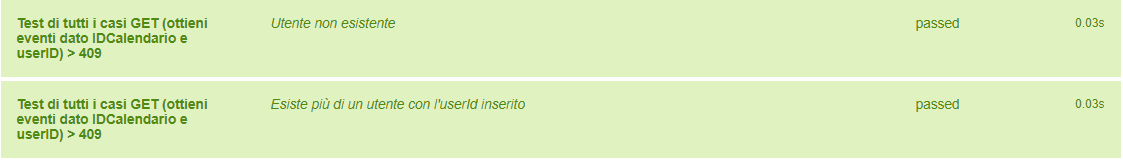
\includegraphics[width=1\textwidth, height=0.09\textheight]{img/png/tests/EventoGet/409_userId_getEventi.png}
                        \blfootnote{Immagine \href{https://github.com/Life-planner/Documentazione/blob/main/D4/img/png/tests/EventoGet/409_userId_getEventi.png}{PNG} Casi 409 riguardo "userId", GET Eventi}
                        \captionof{figure}{Casi 409 riguardo "userId", GET Eventi}
                \end{center}
                Nel penultimo caso siamo andati a testare il caso in cui l' "IDCalendario" non esistesse o  non appartenesse alla lista di calendari dell' "userId" indicato. Da tali casi, bisogna ottenere il codice "409" e il messaggio "There is no calendar with that ID or you are not part of it". Dunque abbiamo inserito un "IDCalendario" inesistente e abbiamo ottenuto, come previsto, il codice e messaggio sopra citati.
                Invece, nell'ultimo caso abbiamo inserito l' "IDCalendario" di un calendario vuoto, che quindi non ci può tornare alcuna lista di eventi, in quanto non l'ha. Dunque, abbiamo creato un calendario vuoto, ottenuto il suo "id" che abbiamo usato come parametro, invocato l'API, aspettandoci che ci ritornasse il codice "409" con il messaggio "There are no events with that userId and IDCalendario", come è successo.
                \begin{center}
                        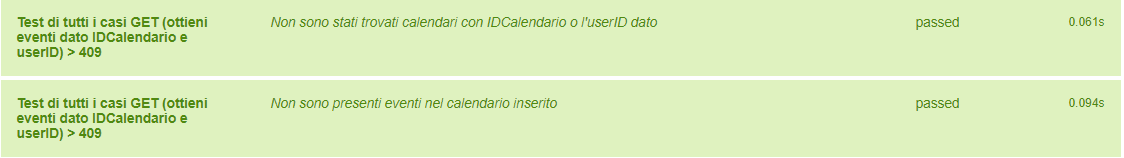
\includegraphics[width=1\textwidth, height=0.09\textheight]{img/png/tests/EventoGet/409_getEventi.png}
                        \blfootnote{Immagine \href{https://github.com/Life-planner/Documentazione/blob/main/D4/img/png/tests/EventoGet/409_getEventi.png}{PNG} Casi 409, GET Eventi}
                        \captionof{figure}{Casi 409, GET Eventi}
                \end{center}
        \elemento [Calendario - POST] {ts:calendarioPost}
                Come già anticipato in \ref{apd:creaCalendario}, lo scopo di questa API è creare e salvare un calendario nel database MongoDB e come già scritto in \ref{apd:creaCalendario}, i parametri minimi necessari affinché questa API possa iniziare la sua procedura sono "userId", "nome" del calendario. Per questo motivo, il primo caso di testing effettuato prende in input solo questi due parametri, scritti in modo tale che siano corretti e che possano superare anche tutti gli altri controlli. Come aspettato, da tale testing otteniamo il codice di risposta "200" con il messaggio "Calendar inserted correctly". Gli altri testing che succedono, che hanno sempre l'obiettivo di ottenere come codice di risposta "200" e "Calendar inserted correctly", non sono altro che dei test in cui abbiamo aggiunto anche gli altri parametri opzionali, ovvero "fusoOrario", "colore" e "principale", in tutte le varie possibili combinazioni. Come si può notare in questa \href{https://plan-it.it/test-report.html} {pagina} e nell'immagine sottostante, anche tutti questi test danno il risultato aspettato per tutti i possibili casi. Abbiamo deciso di fare tutte le possibili combinazioni, anche se non erano del tutto necessario, per fare un'analisi più approfondita, in modo tale che tutti i casi possibili fossero coperti e che nel caso ci fosse stato un errore, questo sarebbe stato individuato e corretto più velocemente.
                \begin{center}
                        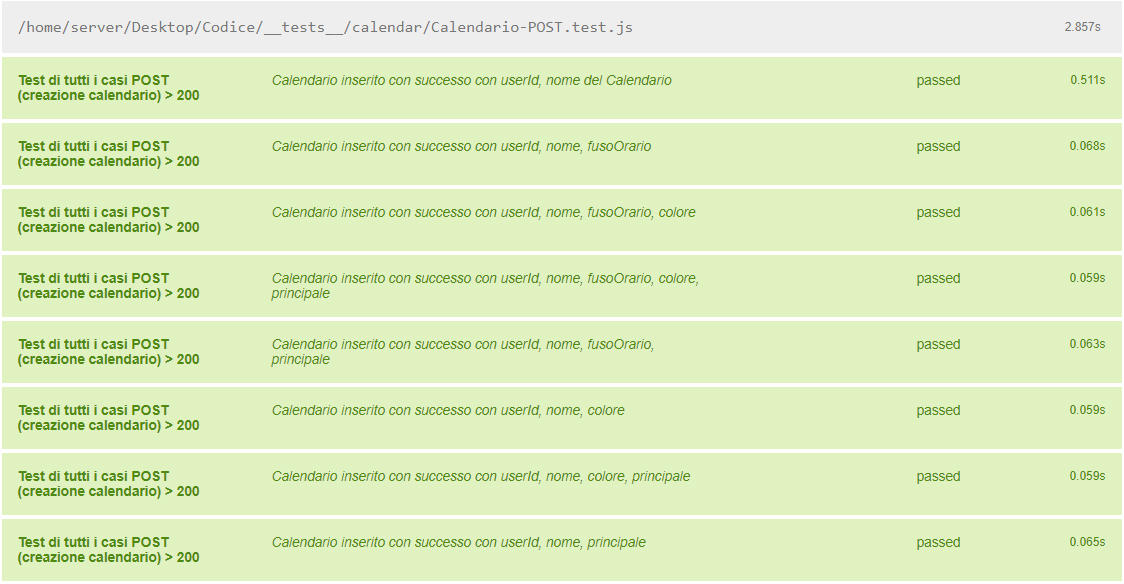
\includegraphics[width=1\textwidth, height=0.42\textheight]{img/png/tests/CalendarioPost/200_postCalendario.png}
                        \blfootnote{Immagine \href{https://github.com/Life-planner/Documentazione/blob/main/D4/img/png/tests/CalendarioPost/200_postCalendario.png}{PNG} Casi 200, POST Calendario}
                        \captionof{figure}{Casi 200, POST Calendario}
                \end{center}
                Dal caso numero 9 al numero 12, i test che andiamo a fare hanno l'obiettivo di ottenere il codice "400" con il messaggio di errore del tipo "Name missing". Per questo motivo, in questi casi mancano in combinazione i parametri "userId" e "nome", parametri, che come detto precedentemente, devono essere sempre presenti affinché questa API possa procedere nell'esecuzione. In tutti questi casi otteniamo, come previsto, il codice "400" con il messaggio di errore "Name missing".
                \begin{center}
                        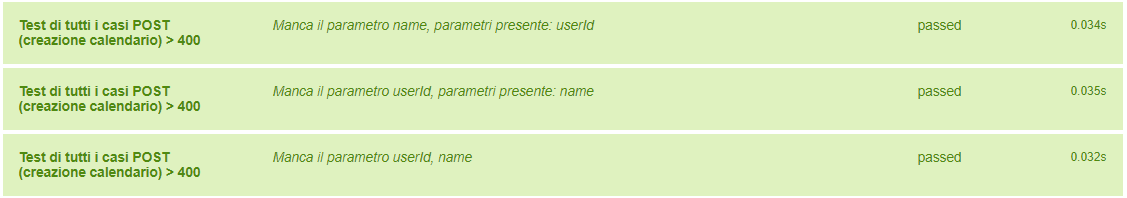
\includegraphics[width=1\textwidth, height=0.13\textheight]{img/png/tests/CalendarioPost/400_missingParameter_PostCalendario.png}
                        \blfootnote{Immagine \href{https://github.com/Life-planner/Documentazione/blob/main/D4/img/png/tests/CalendarioPost/400_missingParameter_CalendarioEvento.png}{PNG} Casi 400 "Name missing", POST Calendario}
                        \captionof{figure}{Casi 400 "Name missing", POST Calendario}
                \end{center}
                Dal caso numero 13 al caso numero 15, abbiamo fatto dei test, che hanno l'obiettivo di ottenere il codice "400" con il messaggio di errore del tipo "Wrong format for (parameter)". Infatti, i seguenti attributi potrebbero avere dei formati sbagliati, ovvero "colore" e "fusoOrario". Questi potrebbero avere dei formati sbagliati e per questo motivo devono essere controllati. Quindi, in questi casi, sono messi tutti i possibili formati erronei per questi parametri, in modo tale da poter osservare che l'API li individui, cosa che succede come aspettato e che si può osservare nella foto sottostante e da questa \href{https://plan-it.it/test-report.html} {pagina}.
                \begin{center}
                        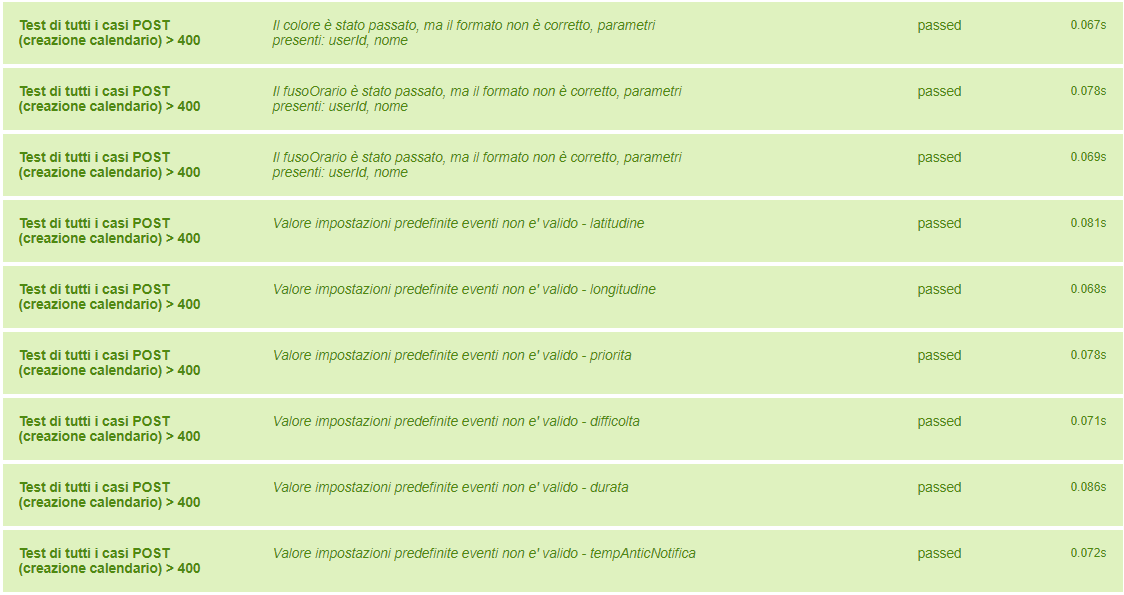
\includegraphics[width=1\textwidth, height=0.13\textheight]{img/png/tests/CalendarioPost/400_wrongFormat_PostCalendario.png}
                        \blfootnote{Immagine \href{https://github.com/Life-planner/Documentazione/blob/main/D4/img/png/tests/CalendarioPost/400_wrongFormat_PostCalendario.png}{PNG} Casi 400 "Wrong format for (parameter)", POST Calendario}
                        \captionof{figure}{Casi 400 "Wrong format for (parameter)", POST Calendario}
                \end{center}
                Infine, negli ultimi casi di test si controlla i casi in cui si inserisse un "userId" non esistente o duplicato, questo venga individuato e sia inviato il codice "409" con i messaggi "There is no user with that userId" e "There is too many users with that userId" rispettivamente. Dati "userId" duplicati o non esistenti otteniamo questi output come previsto e come ne abbiamo già parlato in \ref{ts:eventoPost}. \\
                Invece, un altro caso in cui otteniamo il codice "409", è quello in cui l'utente prova a creare un calendario principale, quando ne ha già uno principale; infatti, ricordiamo, che un utente può avere al massimo un calendario principale alla volta. Per questo motivo, in questo test siamo andati a creare, in primo luogo, un calendario principale per un dato utente esistente: questa procedura va a buon fine e ripetiamo la stessa cosa una seconda volta. La seconda volta, come aspettato, otteniamo il codice "409" con messaggio di errore "There are too many primary calendars".
                \begin{center}
                        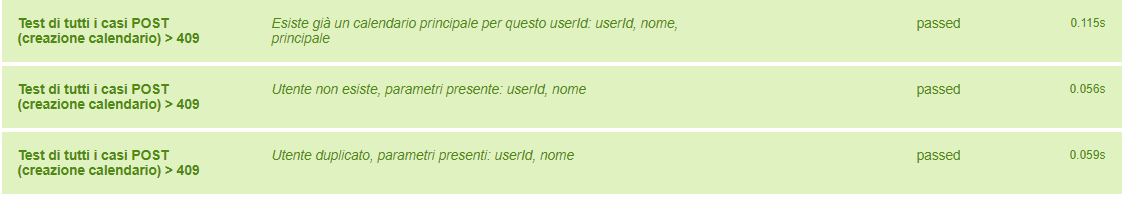
\includegraphics[width=1\textwidth, height=0.12\textheight]{img/png/tests/CalendarioPost/409_postCalendario.png}
                        \blfootnote{Immagine \href{https://github.com/Life-planner/Documentazione/blob/main/D4/img/png/tests/CalendarioPost/409_postCalendario.png}{PNG} Casi 409, POST Calendario}
                        \captionof{figure}{Casi 409, POST Calendario}
                \end{center}
                \newpage
        \elemento [Calendario - PUT] {ts:calendarioPut}
                Questa API, per iniziare la propria di procedura (come già scritto in \ref{apd:modificaCalendario}), ha bisogno di tutti gli attributi che formano una struttura dati "Calendario" come parametri in input, ovvero "IDCalendario", "id" del calendario che si vuole modificare, "nome", nome del calendario, "fusoOrario", "colore", "partecipanti", persone che partecipano agli eventi appartenenti a questo calendario, "principale", booleano che indica se il calendario modificato è quello principale o meno. Quindi nel primo test, in cui avevamo l'obiettivo di ottenere il codice "200" con il messaggio di successo "Calendar modified correctly", abbiamo inserito come parametri tutti questi attributi, in modo che fossero corretti e superassero anche gli altri controlli, e come aspettato, abbiamo ottenuto come codice e messaggio quelli sopra citati.
                \begin{center}
                        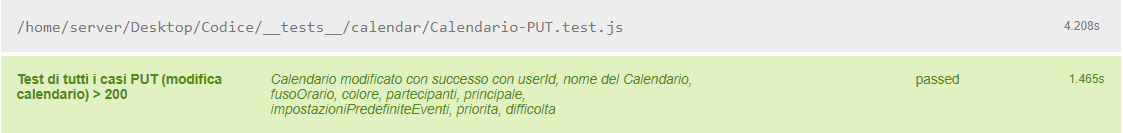
\includegraphics[width=1\textwidth, height=0.08\textheight]{img/png/tests/CalendarioPut/200_putCalendario.png}
                        \blfootnote{Immagine \href{https://github.com/Life-planner/Documentazione/blob/main/D4/img/png/tests/CalendarioPut/200_putCalendario.png}{PNG} Casi 200, PUT Evento}
                        \captionof{figure}{Casi 200, PUT Calendario}
                \end{center}
                Nei seguenti diciannove test avevamo l'obiettivo di ottenere dall'API il codice "400" con il messaggio "Parameter missing"; infatti, siamo andati a togliere, uno alla volta, i parametri sopra scritti, andando anche più nello specifico e togliendo una alla volta anche gli attributi che formavano gli oggetti "luogo" e "impostazioniPredefiniteEventi", per notare se l'API notasse queste mancanze e ci inviasse il codice e messaggio sopra descritti. Come si può notare dalla foto sottostante e da questa \href{https://plan-it.it/test-report.html} {pagina}, così è stato!
                \begin{center}
                        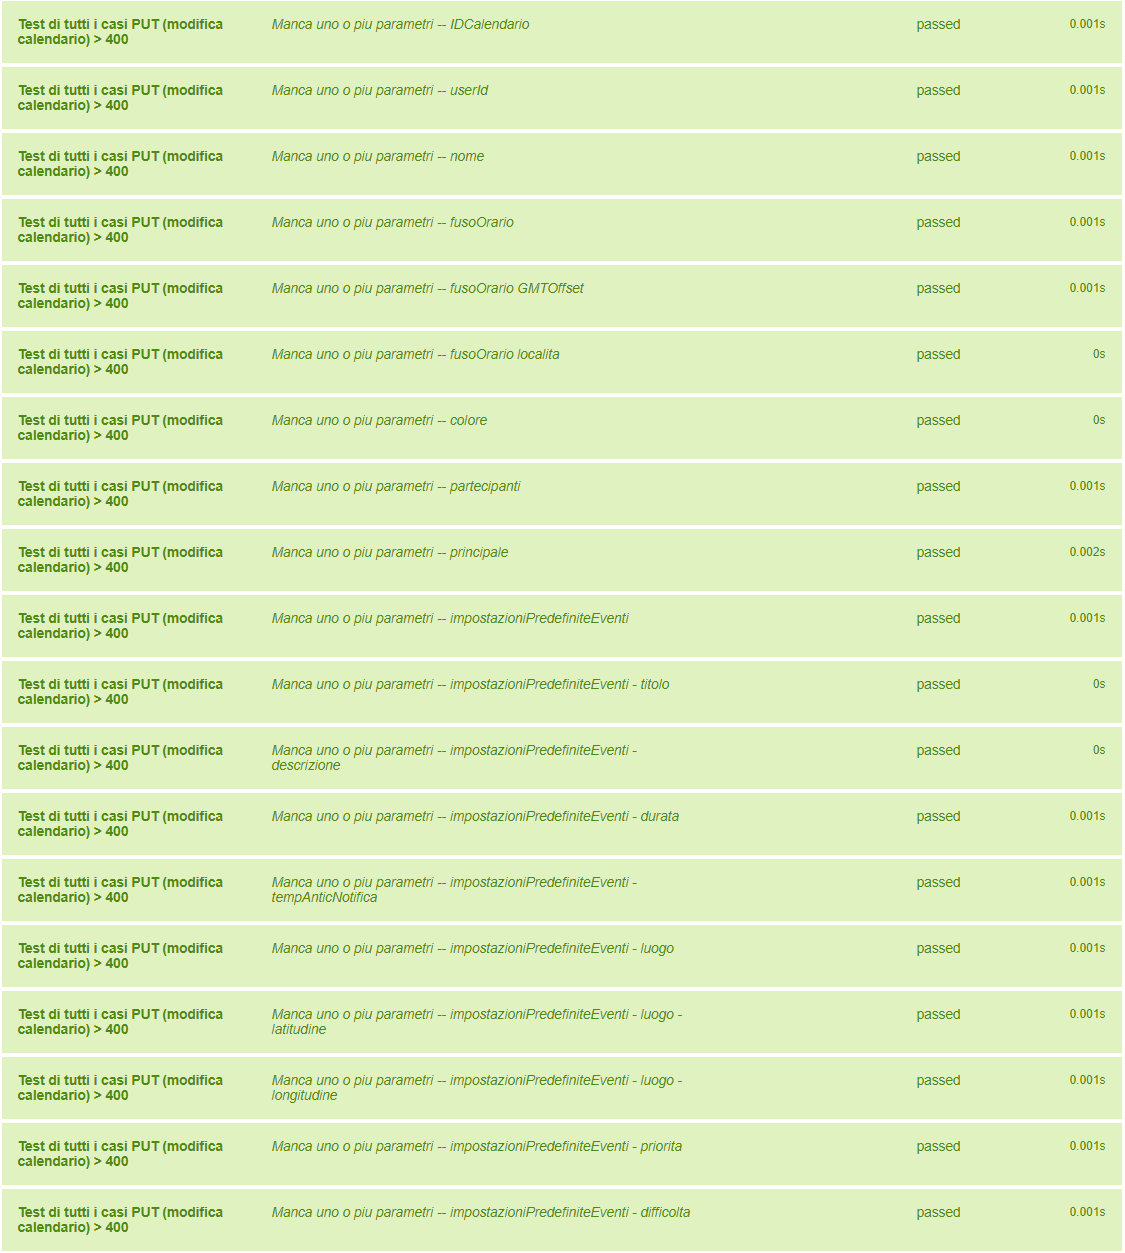
\includegraphics[width=0.73\textwidth, height=0.48\textheight]{img/png/tests/CalendarioPut/400_missingParameter_PutCalendario.png}
                        \blfootnote{Immagine \href{https://github.com/Life-planner/Documentazione/blob/main/D4/img/png/tests/CalendarioPut/400_missingParameter_PutCalendario.png}{PNG} Casi 400, PUT Calendario}
                        \captionof{figure}{Casi 400 "Parameter missing", PUT Calendario}
                \end{center}
                Nei seguenti otto test, siamo andati ad osservare se, nel caso in cui inviassimo dei parametri, una alla volta, con un formato sbagliato, l'API lo notasse e ci inviasse di ritorno il codice "400" con messaggio  "Wrong format for (parameter)". I parametri che possono avere un formato sbagliato sono: "fusoOrario", "colore", attributi "latitudine" e "longitudine" appartenenti all'oggetto "luogo", gli attributi "priorita", "difficolta", "durata", "tempoAnticNotifica" appartenenti all'oggetto "impostazioniPredefiniteEventi". Dunque, abbiamo fatto dei test in cui abbiamo inviato, una alla volta, i parametri sopra citati con dei formati sbagliati e, come aspettato, abbiamo ottenuto il codice "400" con messaggio "Wrong format for (parameter)" in ciascuno dei controlli.
                \begin{center}
                        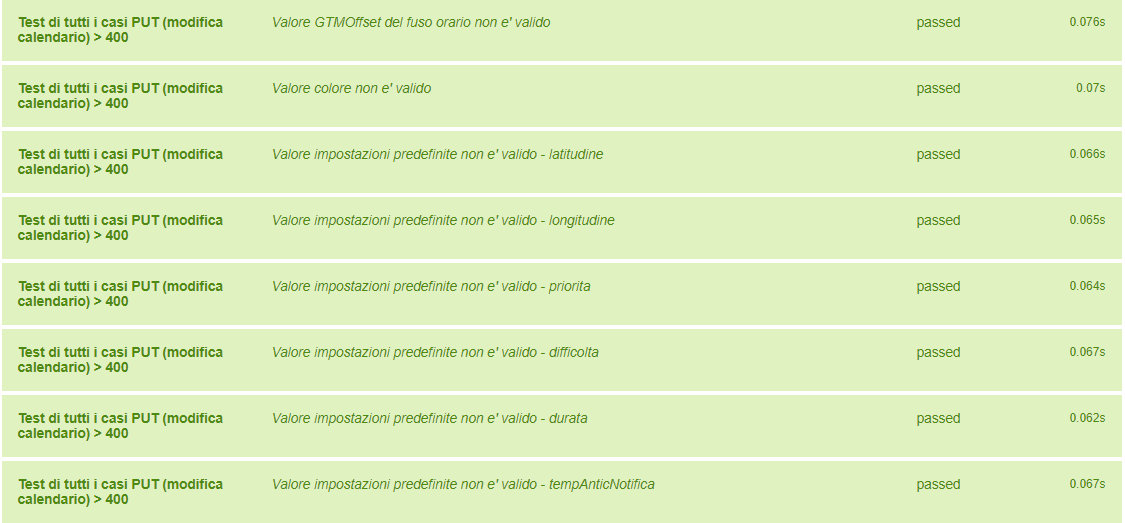
\includegraphics[width=1\textwidth, height=0.28\textheight]{img/png/tests/CalendarioPut/400_wrongFormat_PutCalendario.png}
                        \blfootnote{Immagine \href{https://github.com/Life-planner/Documentazione/blob/main/D4/img/png/tests/CalendarioPut/400_wrongFormat_PutCalendario.png}{PNG} Casi 400 "Wrong format for (parameter)", PUT Calendario}
                        \captionof{figure}{Casi 400 "Wrong format for (parameter)", PUT Calendario}
                \end{center}
                Nei seguenti due casi siamo andati a controllare che l'API notasse, come sempre, i casi in cui l' "userId" è errato, ovvero o duplicato o non esistente, e come negli altri casi abbiamo ottenuto il codice "409" con i messaggi corrispondenti, ovvero "There is no user with that userId" e "There are too many users with that userId" rispettivamente.
                \begin{center}
                        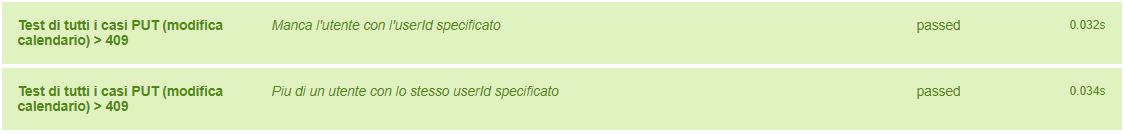
\includegraphics[width=1\textwidth, height=0.08\textheight]{img/png/tests/CalendarioPut/409_userId_PutCalendario.png}
                        \blfootnote{Immagine \href{https://github.com/Life-planner/Documentazione/blob/main/D4/img/png/tests/CalendarioPut/409_userId_PutCalendario.png}{PNG} Casi 409 riguardo "userId", PUT Calendario}
                        \captionof{figure}{Casi 409 riguardo "userId", PUT Calendario}
                \end{center}
                Nell'ultimo caso di test, abbiamo inserito un "IDCalendario" errato, ovvero o non esistente o che non facesse parte della lista di calendari appartenenti a un dato "userId", aspettandoci di ottenere il codice "409" con il messaggio di errore "You do not own the calendar", come è successo.
                \begin{center}
                        \includegraphics[width=1\textwidth, height=0.04\textheight]{img/png/tests/CalendarioPut/409_PutCalendario.png}
                        \blfootnote{Immagine \href{https://github.com/Life-planner/Documentazione/blob/main/D4/img/png/tests/CalendarioPut/409_PutCalendario.png}{PNG} Casi 409, PUT Calendario}
                        \captionof{figure}{Casi 409, PUT Calendario}
                \end{center}
        \elemento [Calendario - DELETE] {ts:calendarioDelete}
                Questa API, come già scritto in \ref{apd:eliminaCalendario}, ha bisogno dell' "IDCalendario" del calendario che si vuole eliminare con l' "userId" dell'utente che ha tale calendario. Dunque, nel primo test, in cui volevamo ottenere il codice "200" con messaggio di successo "Event deleted correctly", abbiamo inserito questi parametri scritti correttamente, che quindi potessero superare anche gli altri controlli presenti nell' API. Come previsto, da questo test abbiamo ottenuto il codice e messaggio sopra scritto.
                \begin{center}
                        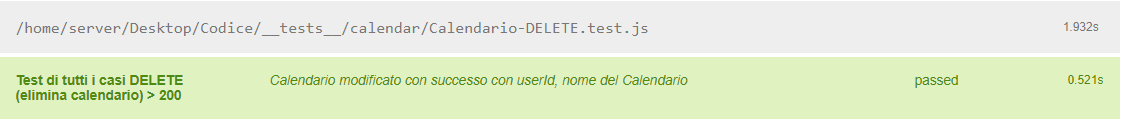
\includegraphics[width=1\textwidth, height=0.08\textheight]{img/png/tests/CalendarioDelete/200_deleteCalendario.png}
                        \blfootnote{Immagine \href{https://github.com/Life-planner/Documentazione/blob/main/D4/img/png/tests/CalendarioDelete/200_DeleteCalendario.png}{PNG} Casi 200, DELETE Calendario}
                        \captionof{figure}{Casi 200, DELETE Calendario}
                \end{center}
                Nei seguenti casi, siamo andati a controllare che nel caso in cui, non inserissimo uno dei parametri sopra citati, l'API lo notasse e ci inviasse il codice "400" con messaggio di errore "Parameter missing", cosa che è avvenuta sia nel caso in cui mancava "userId", sia nel caso in cui mancava "IDCalendario" e sia nel caso in cui mancavano entrambi.
                \begin{center}
                        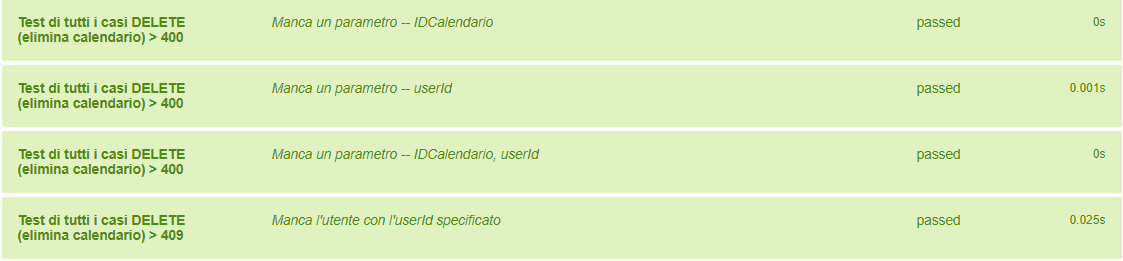
\includegraphics[width=1\textwidth, height=0.15\textheight]{img/png/tests/CalendarioDelete/400_missingParameter_deleteCalendario.png}
                        \blfootnote{Immagine \href{https://github.com/Life-planner/Documentazione/blob/main/D4/img/png/tests/CalendarioDelete/400_missingParameter_deleteCalendario.png}{PNG} Casi 400 "Parameter missing", DELETE Calendario}
                        \captionof{figure}{Casi 400 "Parameter missing", DELETE Calendario}
                \end{center}
                In seguito, abbiamo fatto, come in \ref{ts:eventoPost}, i due test in cui inseriamo un "userId" scorretto, ovvero o duplicato o non esistente, aspettandoci il codice "409" con i messaggi "There are too many users with that userId" e "There is no user with that userId" rispettivamente. E, come avvenuto in \ref{ts:eventoPost}, i due test sono avvenuti con successo, ottenendo i codici e messaggi sopra citati.
                \begin{center}
                        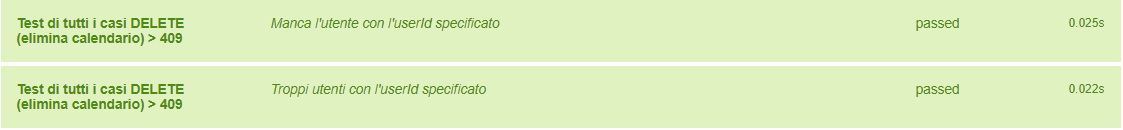
\includegraphics[width=1\textwidth, height=0.08\textheight]{img/png/tests/CalendarioDelete/409_userId_deleteCalendario.png}
                        \blfootnote{Immagine \href{https://github.com/Life-planner/Documentazione/blob/main/D4/img/png/tests/CalendarioDelete/409_userId_deleteCalendario.png}{PNG} Casi 409 riguardo "userId", DELETE Calendario}
                        \captionof{figure}{Casi 409 riguardo "userId", DELETE Calendario}
                \end{center}
                L'ultimo caso testato è quello in cui si inserisce un "IDCalendario" che non esiste tra gli "id" dei calendari appartenenti all' "userId" dato. In questo caso, prevediamo di ottenere il codice "409" con il messaggio di errore "You do not own the calendar", cosa che è avvenuta; quindi, anche questo test è andato a buon fine.
                \begin{center}
                        \includegraphics[width=1\textwidth, height=0.04\textheight]{img/png/tests/EventoDelete/409_DeleteEvento.png}
                        \blfootnote{Immagine \href{https://github.com/Life-planner/Documentazione/blob/main/D4/img/png/tests/EventoDelete/409_DeleteEvento.png}{PNG} Casi 409, DELETE Evento}
                        \captionof{figure}{Casi 409, DELETE Evento}
                \end{center}

        \elemento [Calendari - GET] {ts:calendariGet}
                Già anticipato in precedenza in \ref{apd:getCalendari}, lo scopo di questa API è ottenere tutti i calendari di un utente autenticato. Dunque, l'unico parametro che deve essere sempre presente, affinché l'API possa avere successo, se passa anche i successivi controlli, è l' "userId" dell'utente autenticato. Per questo motivo, sono stati effettuati solo due test, da cui ci si aspetta di ottenere successo con codice "200" e l'array di calendari. Il primo test è stato effettuato passando l' "userId" di un utente che ha solo un calendario personale, invece il secondo con un "userId" che ha due calendari personali. Come si può notare dalla foto sottostante a da questa \href{https://plan-it.it/test-report.html} {pagina}, questi due test hanno avuto il risultato aspettato.
                \begin{center}
                        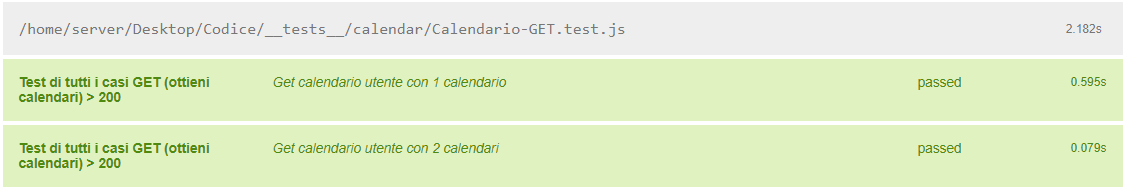
\includegraphics[width=1\textwidth, height=0.1\textheight]{img/png/tests/CalendarioGet/200_getCalendari.png}
                        \blfootnote{Immagine \href{https://github.com/Life-planner/Documentazione/blob/main/D4/img/png/tests/CalendarioGet/200_getCalendari.png}{PNG} Casi 200, GET Calendari}
                        \captionof{figure}{Casi 200, GET Calendari}
                \end{center}
                In seguito, abbiamo testato che l'API notasse il caso in cui non inserissimo l'unico parametro richiesto, ovvero "userId". Come aspettato, come si può notare dalla foto sottostante e anche da questa \href{https://plan-it.it/test-report.html} {pagina}, l'API ha dato la risposta aspettata, inviando come output il codice "400" con messaggio "Parameter missing".
                \begin{center}
                        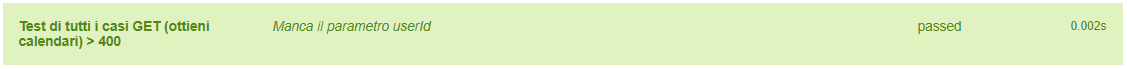
\includegraphics[width=1\textwidth, height=0.04\textheight]{img/png/tests/CalendarioGet/400_getCalendari.png}
                        \blfootnote{Immagine \href{https://github.com/Life-planner/Documentazione/blob/main/D4/img/png/tests/CalendarioGet/400_getCalendari.png}{PNG} Casi 400 "Parameter missing", GET Calendari}
                        \captionof{figure}{Casi 400 "Parameter missing", GET Calendari}
                \end{center}
                Dopo si è passati a controllare il caso in cui si inserisse il parametro "userId" incorretto, ovvero non esistente nel database o duplicato, l'API individui tale errore e restituisca il codice "409" con il relativo messaggio. Infatti, quando abbiamo inserito l' "userId" di un utente non esistente, l'API ha individuato tale errore restituendo "409 - There is no user with that userId". Invece, nel secondo caso, (abbiamo sempre creato un userId duplicato all'inizio della procedura di testing come fatto in \ref{ts:eventoPost}) con l'inserimento di un "userId" duplicato, abbiamo ottenuto come ci si aspettava, l'errore "409 - There are too many users with that userId".
                Infine, abbiamo controllato il caso in cui inviassimo, come parametro, l' "userId" di un utente che non avesse alcun calendario; in questo ci aspettiamo il codice "409" con il messaggio di errore "There are no calendars with that userId". Come si può notare, anche questo test è andato a buon fine; infatti abbiamo ottenuto  quello previsto.
                \begin{center}
                        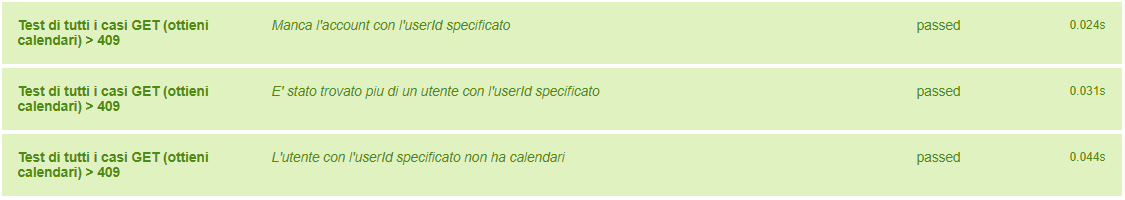
\includegraphics[width=0.87\textwidth, height=0.09\textheight]{img/png/tests/CalendarioGet/409_getCalendari.png}
                        \blfootnote{Immagine \href{https://github.com/Life-planner/Documentazione/blob/main/D4/img/png/tests/CalendarioGet/409_getCalendari.png}{PNG} Casi 409, GET Calendari}
                        \captionof{figure}{Casi 409, GET Calendari}
                \end{center}
        \elemento [Utente - POST] {ts:utentePost}
                Come già anticipato in \ref{apd:creaAccount}, questa API, per iniziare il suo processo di creazione di un utente nel database, ha bisogno dei seguenti parametri: "userId", "email" ed "username". Dunque, nel primo test abbiamo messo questi parametri corretti in input, aspettandoci di ottenere il codice "200" con messaggio "User inserted correctly", cosa, che come si può notare dalla foto sottostante e da questa \href{https://plan-it.it/test-report.html} {pagina}, è avvenuta.
                \begin{center}
                        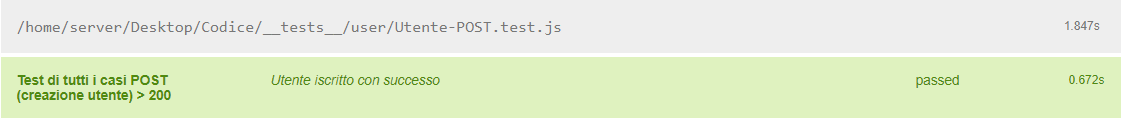
\includegraphics[width=1\textwidth, height=0.08\textheight]{img/png/tests/UtentePost/200_postUtente.png}
                        \blfootnote{Immagine \href{https://github.com/Life-planner/Documentazione/blob/main/D4/img/png/tests/UtentePost/200_postUtente.png}{PNG} Casi 200, POST Utente}
                        \captionof{figure}{Casi 200, POST Utente}
                \end{center}
                Nei seguenti test, siamo andati a controllare i casi in cui mancassero uno o più parametri di quelli sopra citati, in tutte le possibili combinazioni, in modo tale da poter osservare se l'API si comportasse nel modo corretto in ogni caso. Ci aspettavamo, in ciascun caso, il codice "400" con il messaggio di errore "Parameter missing", cosa che è successa.
                \begin{center}
                        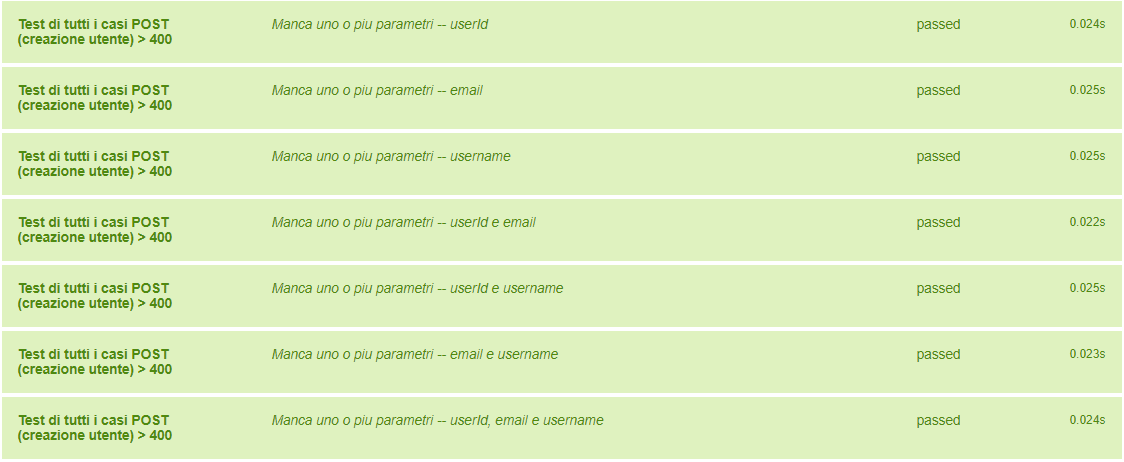
\includegraphics[width=1\textwidth, height=0.25\textheight]{img/png/tests/UtentePost/400_missingParameter_PostUtente.png}
                        \blfootnote{Immagine \href{https://github.com/Life-planner/Documentazione/blob/main/D4/img/png/tests/UtentePost/400_missingParameter_PostUtente.png}{PNG} Casi 400 "Parameter missing", POST Utente}
                        \captionof{figure}{Casi 400 "Parameter missing", POST Utente}
                \end{center}
                Nell'ultimo caso, controllato per questa API, abbiamo messo dei parametri che corrispondessero ad un utente già esistente, ovvero l' "userId" era già esistente nel database MongoDB. Nel caso in cui si provasse a creare un utente già esistente, questa API dovrebbe rispondere con codice "409" e messaggio "There is already one user with that id or email", cosa che è avvenuta come previsto.
                \begin{center}
                        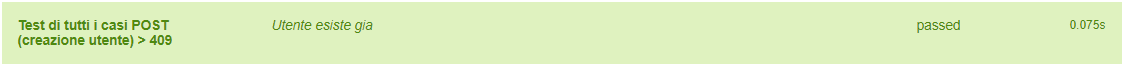
\includegraphics[width=1\textwidth, height=0.05\textheight]{img/png/tests/UtentePost/409_postUtente.png}
                        \blfootnote{Immagine \href{https://github.com/Life-planner/Documentazione/blob/main/D4/img/png/tests/UtentePost/409_postUtente.png}{PNG} Casi 409, POST Utente}
                        \captionof{figure}{Casi 409, POST Utente}
                \end{center}
        \elemento [Utente - PUT] {ts:utentePut}
                Questa API, come già scritto in \ref{apd:modificaAccount}, ha lo scopo di modificare l' "username" di un utente identificato dal suo "userId". Per questo motivo, i parametri che devono essere presenti quando si invoca questa API, sono i due attributi sopra citati. Dunque, nel primo test, in cui volevamo ottenere il codice "200" e il messaggio di successo "User update correctly", abbiamo inserito questi due parametri in modo che superassero anche gli altri controlli presenti e, come previsto, abbiamo ottenuto il codice e messaggio scritti precedentemente.
                \begin{center}
                        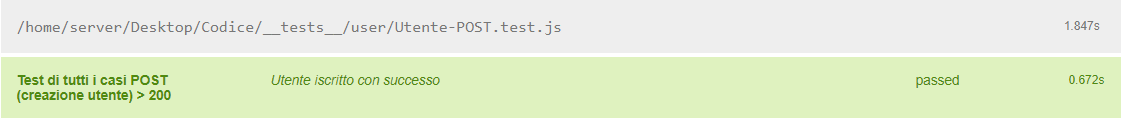
\includegraphics[width=1\textwidth, height=0.08\textheight]{img/png/tests/UtentePost/200_postUtente.png}
                        \blfootnote{Immagine \href{https://github.com/Life-planner/Documentazione/blob/main/D4/img/png/tests/UtentePost/200_postUtente.png}{PNG} Casi 200, POST Utente}
                        \captionof{figure}{Casi 200, POST Utente}
                \end{center}
                Nei seguenti casi, siamo andati a controllare che, se non inserissimo uno dei parametri sopra descritti, l'API lo nota e ci invii il codice "400" con messaggio di errore "Parameter missing", cosa che è avvenuta sia nel caso in cui mancava "userId", sia nel caso in cui mancava "username" e sia nel caso in cui mancavano entrambi.
                \begin{center}
                        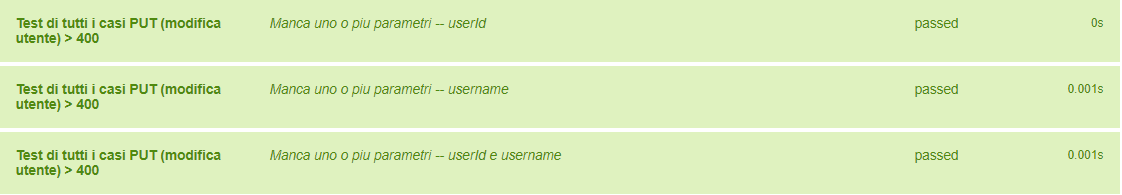
\includegraphics[width=1\textwidth, height=0.13\textheight]{img/png/tests/UtentePut/400_missingParameter_putUtente.png}
                        \blfootnote{Immagine \href{https://github.com/Life-planner/Documentazione/blob/main/D4/img/png/tests/UtentePut/400_missingParameter_putUtente.png}{PNG} Casi 400 "Parameter missing", PUT Utente}
                        \captionof{figure}{Casi 400 "Parameter missing", PUT Utente}
                \end{center}
                Negli ultimi due casi siamo andati a controllare che l'API notasse, come sempre, i casi in cui l' "userId" inviato in input fosse errato, ovvero o duplicato o non esistente, e, come nelle altre APIs, abbiamo ottenuto il codice "409" con i messaggi corrispondenti, ovvero "There is no user with that userId" e "There are too many users with that userId" rispettivamente.
                \begin{center}
                        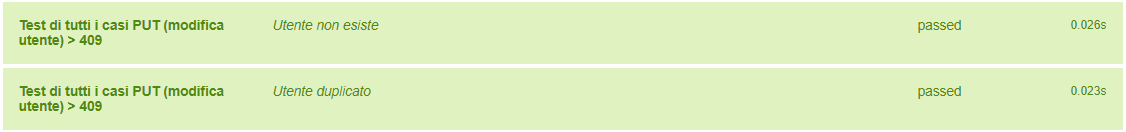
\includegraphics[width=1\textwidth, height=0.08\textheight]{img/png/tests/UtentePut/409_userId_putUtente.png}
                        \blfootnote{Immagine \href{https://github.com/Life-planner/Documentazione/blob/main/D4/img/png/tests/UtentePut/409_userId_putUtente.png}{PNG} Casi 409, PUT Utente}
                        \captionof{figure}{Casi 409, PUT Utente}
                \end{center}
                \newpage
        \elemento [Utente - GET-Email] {ts:utenteGetEmail}
                Questa API, come già descritto in \ref{apd:getDatiAccount_email}, ha bisogno di un' "email" per poter identificare un utente all'interno del database MongoDB; dunque l' "email" è l'unico parametro necessario. Nel primo test, abbiamo inserito un' "email" corretta aspettandoci di ottenere, come ritorno, il codice "200" e l'oggetto "UtenteAutenticato" dell'utente che ha tale "email", cosa che è avvenuta.
                \begin{center}
                        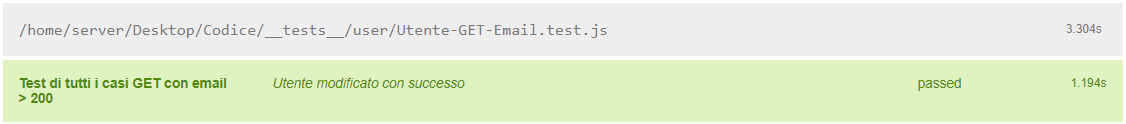
\includegraphics[width=1\textwidth, height=0.08\textheight]{img/png/tests/UtenteGet_email/200_getUtente_email.png}
                        \blfootnote{Immagine \href{https://github.com/Life-planner/Documentazione/blob/main/D4/img/png/tests/UtenteGet_email/200_getUtente_email.png}{PNG} Casi 200,  Get Utente\_email}
                        \captionof{figure}{Casi 200, Get Utente\_email}
                \end{center}
                Nel secondo test effettuato non abbiamo inserito nessun parametro, ovvero non abbiamo messo l' "email". Dunque l'API non può procedere, ma prevediamo invii il codice "400" con il messaggio di errore "Parameter missing", cosa che accade.
                \begin{center}
                        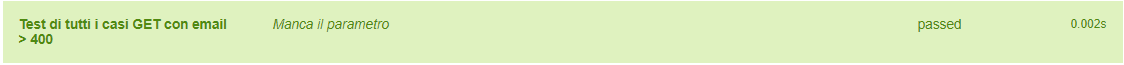
\includegraphics[width=1\textwidth, height=0.04\textheight]{img/png/tests/UtenteGet_email/400_missingParameter_getUtente_email.png}
                        \blfootnote{Immagine \href{https://github.com/Life-planner/Documentazione/blob/main/D4/img/png/tests/UtenteGet_email/400_missingParameter_getUtente_email.png}{PNG} Casi 400 "Parameter missing", Get Utente\_email}
                        \captionof{figure}{Casi 400 "Parameter missing", Get Utente\_email}
                \end{center}
                Gli ultimi due casi sono quelli in cui inseriamo un' "email" scorretta, ovvero o non esistente o duplicata; dunque ci aspettiamo il codice "409" con il messaggio di errore "There is no user with that email" e "There are too many users with that email" rispettivamente. Come possiamo notare nella foto sottostante, o da questa \href{https://plan-it.it/test-report.html} {pagina}, anche questi test hanno avuto esito positivo.
                \begin{center}
                        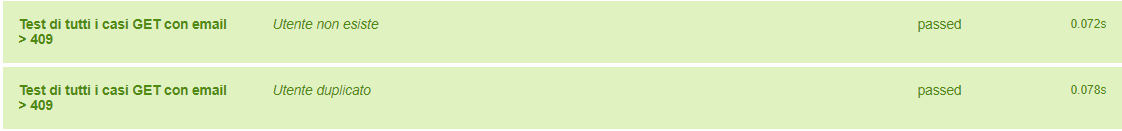
\includegraphics[width=1\textwidth, height=0.08\textheight]{img/png/tests/UtenteGet_email/409_userId_getUtente_email.png}
                        \blfootnote{Immagine \href{https://github.com/Life-planner/Documentazione/blob/main/D4/img/png/tests/UtenteGet_email/409_userId_getUtente_email.png}{PNG} Casi 409, Get Utente\_email}
                        \captionof{figure}{Casi 409, Get Utente\_email}
                \end{center}
                \newpage
        \elemento [Utente - GET-UserId] {ts:utenteGetUserId}
                Per questa API sono stati fatti gli test già presentati sopra in "Utente - GET-Email" (\ref{ts:utenteGetEmail}), con l'unica differenza che al posto dell' "email", abbiamo l' "userId". Dunque non ripetiamo la descrizione dei casi, in quanto sono gli stessi, ma con l' "userId".
                \begin{center}
                        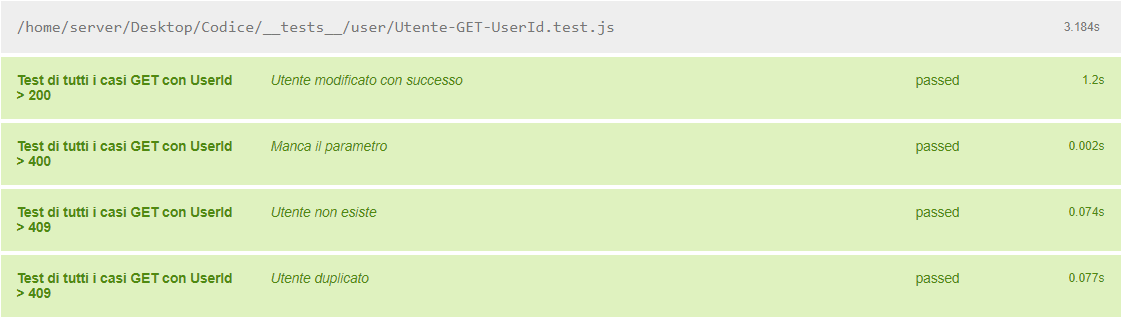
\includegraphics[width=1\textwidth, height=0.2\textheight]{img/png/tests/UtenteGet_userId/getUtente_userId.png}
                        \blfootnote{Immagine \href{https://github.com/Life-planner/Documentazione/blob/main/D4/img/png/tests/UtenteGet_userId/getUtente_userId.png}{PNG} Casi 200, GET Utente\_userId}
                        \captionof{figure}{Casi 200, GET Utente\_userId}
                \end{center}
\end{listaPersonale}